\documentclass[a4paper,11pt]{article}
\input{/home/tof/Documents/Cozy/latex-include/preambule_lua.tex}
\newcommand{\showprof}{show them}  % comment this line if you don't want to see todo environment
\fancyhead[L]{Formulaire web}
\newdate{madate}{10}{09}{2020}
%\fancyhead[R]{\displaydate{madate}} %\today
%\fancyhead[R]{Seconde - SNT}
\fancyhead[R]{Première - NSI}
%\fancyhead[R]{Terminale - NSI}
\fancyfoot[L]{~\\Christophe Viroulaud}
\AtEndDocument{\label{lastpage}}
\fancyfoot[C]{\textbf{Page \thepage/\pageref{lastpage}}}
\fancyfoot[R]{\includegraphics[width=2cm,align=t]{/home/tof/Documents/Cozy/latex-include/cc.png}}

\begin{document}
\begin{Form}
\begin{commentprof}
Mettre premier-formulaire.zip sur site
\end{commentprof}
\section{Problématique}
Une action indispensable pour un site marchand est de pouvoir recueillir des informations de la part de ses clients. Il doit par exemple récupérer l'adresse de l'acheteur pour pouvoir lui livrer ses achats. Cette prise d'informations se réalise par le biais de \emph{formulaires}.
\begin{center}
 \shadowbox{\parbox{12cm}{\centering Comment mettre en place un formulaire sur un site web?}}
 \end{center}
\section{Création du formulaire}
\subsection{Éléments de base}
Les formulaires HTML permettent à l'utilisateur d'envoyer des données au site web. Ils sont donc composés a minima d'un \emph{champ} que l'utilisateur devra remplir et d'un \emph{bouton d'envoi} pour transmettre les données. La balise HTML \emph{form} permet de créer un formulaire. Chaque champ sera crée avec une balise \emph{input}.
\begin{activite}
\begin{enumerate}
\item Créer une page web puis insérer le code \ref{formulaire} entre les balises \emph{body}.
\begin{center}
\begin{lstlisting}[language=HTML]
<form>
   <input type="text">
   <input type="password">
   <input type="submit" value="Envoyer">
</form>
\end{lstlisting}
\captionof{code}{Premier formulaire}
\label{formulaire}
\end{center}
\item Visualiser la page web dans un navigateur.
\item Écrire dans chacun des deux champs et observer les différences. Comment les expliquer?
\end{enumerate}
\end{activite}
Il existe de nombreux types de champs prédéfinis. La page \mbox{\url{https://tinyurl.com/yb45a39q}} recense les possibilités.
\subsection{Soigner l'esthétique}
Comme pour tout élément HTML, il est possible d'habiller un formulaire avec une page CSS. Le code \ref{habillage} englobe le champ \emph{input} dans une balise \emph{div} à laquelle on applique une classe CSS. De plus une étiquette (\emph{label}) est liée à ce champ.
\begin{center}
\begin{lstlisting}[language=HTML]
<div class="form-securite">
   <label for="nom">Identifiant </label>
   <input type="text" id="nom">
</div>
\end{lstlisting}
\captionof{code}{Habillage d'un champ du formulaire}
\label{habillage}
\end{center}
\begin{activite}
\begin{enumerate}
\item Télécharger le dossier compressé \emph{activite2-identification.zip} sur le site \mbox{\url{https://cviroulaud.github.io}}.
\item Dans le dossier \emph{activite2-identification} observer le code de la page \emph{identification.html} et de la feuille CSS associée (le fichier \emph{traitement.php} ne sera pas utilisé dans cette activité).
\item Quel est le rôle de l'attribut \emph{required}?
\item En s'appuyant sur le modèle précédent, créer le formulaire (figure \ref{livraison}) d'un site marchand.
\begin{center}
\centering
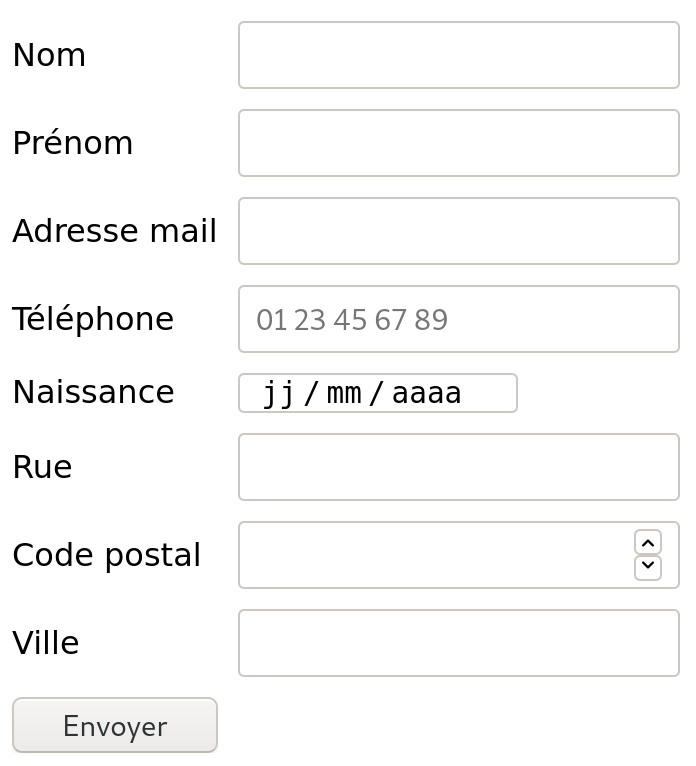
\includegraphics[width=6cm]{ressources/livraison.png}
\captionof{figure}{Page de livraison}
\label{livraison}
\end{center}
\end{enumerate}
\end{activite}
\section{Envoi des données}
\subsection{Principe de fonctionnement}
Pour l'instant le fait d'appuyer sur le bouton de validation ne provoque rien (à part recharger la page). Que doit-il se passer quand un formulaire est validé?
\begin{itemize}
\item Les données sont envoyées au serveur qui héberge le site web.
\begin{center}
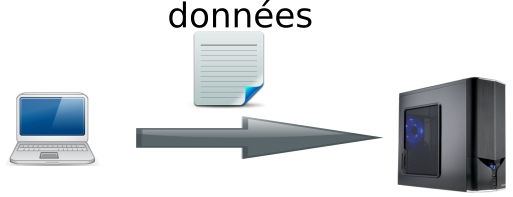
\includegraphics[width=5cm]{ressources/form1.png}
\end{center}
\item Un fichier (souvent en langage \emph{PHP: acronyme récursif pour PHP Hypertext Preprocessor}) traite les données. Il peut stocker les informations dans une base de données, construire une page web personnalisée en fonction des informations...
\begin{center}

\includegraphics[width=5cm]{ressources/form2.png}
\end{center}
\item Le serveur renvoie une page web qui utilise éventuellement les données du formulaire.
\begin{center}
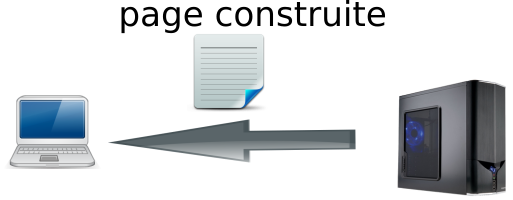
\includegraphics[width=5cm]{ressources/form3.png}
\end{center}
\end{itemize}
Ce fonctionnement implique plusieurs conditions:
\begin{itemize}
\item Il est nécessaire de disposer d'un serveur distant pour pouvoir lui envoyer les données.
\item Le formulaire doit être légèrement modifié pour qu'il sache quelle action réaliser.
\end{itemize} 
\begin{activite}
\begin{enumerate}
\item Se rendre sur le site \url{https://tinyurl.com/y78f4jmp} . Ce serveur distant remplira la première condition.
\item Observer le \emph{code source} de la page web affichée. Quels sont les éléments ajoutés par rapport à l'activité 2?
\end{enumerate}
\end{activite}
\begin{aretenir}[]
\begin{itemize}
\item L'attribut \emph{action} de la balise \emph{form} cible le fichier qui s'occupera du traitement des données. 
\item Les champs \emph{input} doivent contenir un attribut \emph{name}. C'est lui qui sera utilisé par le fichier de traitement.
\end{itemize}
\end{aretenir}
\subsection{Méthodes d'envoi}
Il existe deux méthodes d'envoi des données: GET et POST.
\subsubsection{GET}
\begin{activite}
\begin{enumerate}
\item Sur le site web précédent, compléter le formulaire avec des informations fictives, puis valider.\\
Le site renvoie une page web qui utilise les informations.
\item Observer la barre d'adresse du navigateur. Que peut-on dire à propos de la sécurité de cette méthode d'envoi?
\end{enumerate}
\end{activite}
\begin{aretenir}[]
La méthode \emph{GET} ajoute les données à l'URL. C'est la méthode d'envoi par défaut quand rien n'est précisé dans le formulaire.\\ Ce procédé simple peut poser des problèmes de sécurité. 
\end{aretenir}
\subsubsection{POST}
Il faut préciser la méthode d'envoi avec l'attribut \emph{method} (code \ref{post}).
\begin{center}
\begin{lstlisting}[language=HTML]
<form action="traitement.php" method="post">
\end{lstlisting}
\captionof{code}{Méthode d'envoi}
\label{post}
\end{center}
Les données sont envoyés au serveur dans le corps du message.
\begin{activite}
\begin{enumerate}
\item Se rendre à l'adresse \url{https://tinyurl.com/y8qxp97p}.
\item Observer le code source de la page.
\item Remplir le formulaire avec des données fictives et valider.
\item Dans le dossier \emph{activite2-identification}, observer le code de la page traitement.php
\end{enumerate}
\end{activite}
\begin{aretenir}[Remarque]
L'apprentissage du langage PHP ne fait pas partie du programme de première. La page \emph{traitement.php} est donnée à titre d'observation.
\end{aretenir}
\begin{aretenir}[]
La méthode \emph{POST} doit être précisé dans l'entête du formulaire. Les données sont envoyées dans le corps du message. Il n'y a donc pas de taille limite.\\
\textbf{L'utilisation de cette méthode ne signifie pas que le message est sécurisé: en effet, le contenu circule en clair sur internet. S'il est intercepté, il peut être lu sans difficulté.}
\end{aretenir}
\begin{activite}
\begin{enumerate}
\item Se rendre à nouveau à l'adresse \url{https://tinyurl.com/y8qxp97p}.
\item Entrer un identifiant et un mot de passe fictifs. \emph{Ne pas valider tout de suite.}
\\Choisir le raccourci en fonction du navigateur:
\item \textbf{Sur Firefox:}
\begin{enumerate}
\item  Cliquer sur \emph{Ctrl+Shift+E}, le panneau \emph{réseau} s'ouvre.
\item Dans la page web, valider le formulaire.
\item Ouvrir la ligne \emph{POST}.
\begin{center}
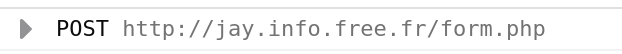
\includegraphics[width=7cm]{ressources/post-ff.png}
\end{center}
\item Dans \emph{Requêtes}, retrouver alors les informations transmises.
\end{enumerate}
\item \textbf{Sur Chrome:}
\begin{enumerate}
\item  Cliquer sur \emph{Ctrl+Shift+I}, un panneau s'ouvre.
\item Choisir \emph{Réseau} ou \emph{Network}.
\item Dans la page web, valider le formulaire.
\item Cliquer sur \emph{form.php}.
\begin{center}
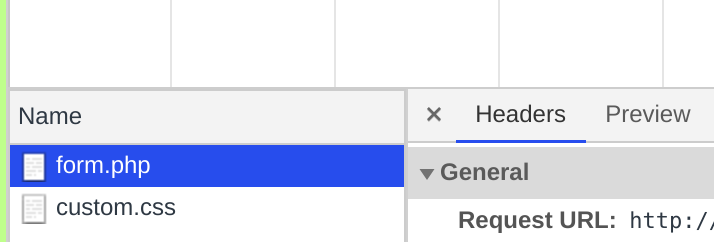
\includegraphics[width=6.5cm]{ressources/post-chrome.png}
\end{center}
\item Dans \emph{Headers}, retrouver alors les informations transmises.
\end{enumerate}
\end{enumerate}
\end{activite}
\end{Form}
\end{document}